%!TEX root = ../main.tex
% file: problem2.tex
\section{Tkinter GUI for Adjacency Matrix} % (fold)
\label{sec:tkinter_gui_for_adjacency_matrix}
We wish to create a random adjacency matrix which carries the form
\begin{equation} \label{eq:A}
    A = \begin{pmatrix} 0 & B \\ B^T & 0 \end{pmatrix}.
\end{equation}
The coefficients $B$ are boolean integers representative of whether or not the index $i$ and $j$ are connected. We then wish to create a unit circle on a Tkinter canvas with vertices located at the coordinates $(cos(2k\pi/n),sin(2k\pi/n))$, where $k$ is the vertex number, and $n$ is the total number of vertices. After creation of the aforementioned unit circle and adjacency matrix, we connect the edges in Eq. \ref{eq:A} with lines on the canvas.

\subsection{Program Description} % (fold)
\label{sub:program_description3}
The script for Problem 3 is divided into two files. The first contains the reusable functions \emph{ranSymMatrix} and \emph{genVertList}. The second file contains the GUI specific operations. 

\begin{lstlisting}[caption={Generation of a Random Adjacency Matrix}, label=lst:ranSym,firstnumber=4]
    def ranSymMatrix(n):
        """Creates a symmetric random matrix """
        arr = numpy.random.random_integers(0,1,size=(n,n))
        for x in range(len(arr)):
            arr[x,x] = 0
        return (arr + arr.T)//2
\end{lstlisting}\noindent
In Listing \ref{lst:ranSym} we generate a random matrix of zeros and ones on line 6. We then set all trace elements to zero, and finally mirror the top of the matrix over the diagonal. We then have a random symmetric matrix with zero diagonals.

\begin{lstlisting}[caption={Main GUI Button Logic}, label=lst:mainGui,firstnumber=33]
    def mainLogic(self):
        """Main execution loop when button is pressed"""
        self.canvas.delete('all')
        n = int(self.nEntry.get())
        
        self.vert = vert = genVertList(n)
        self.drawPoints(vert)
        
        self.conMat = conMat = ranSymMatrix(n)
        self.calcConn(conMat)
\end{lstlisting}\noindent
Our main logic when the button pressed is shown in Listing \ref{lst:mainGui}. We begin by clearing the canvas to ensure no previous results are displayed. We then evaluate the string in the entry box and cast it to an integer. The function $genVertList$ generates $n$ vertices on a unit circle. These vertices are then drawn on the canvas using \emph{drawPoints}. The next step is to generate our adjacency matrix, and pass it to the function \emph{calcConn}, which calculates which vertices are connected and draws a line between them.
% subsection program_description (end)


\subsection{Results} % (fold)
\label{sub:results3}
As a test we run the script and ensure the that proper vertices are connected with edges. We also print out the corresponding adjacency matrix to verify the connections.
\begin{figure}[H]
    \centering
        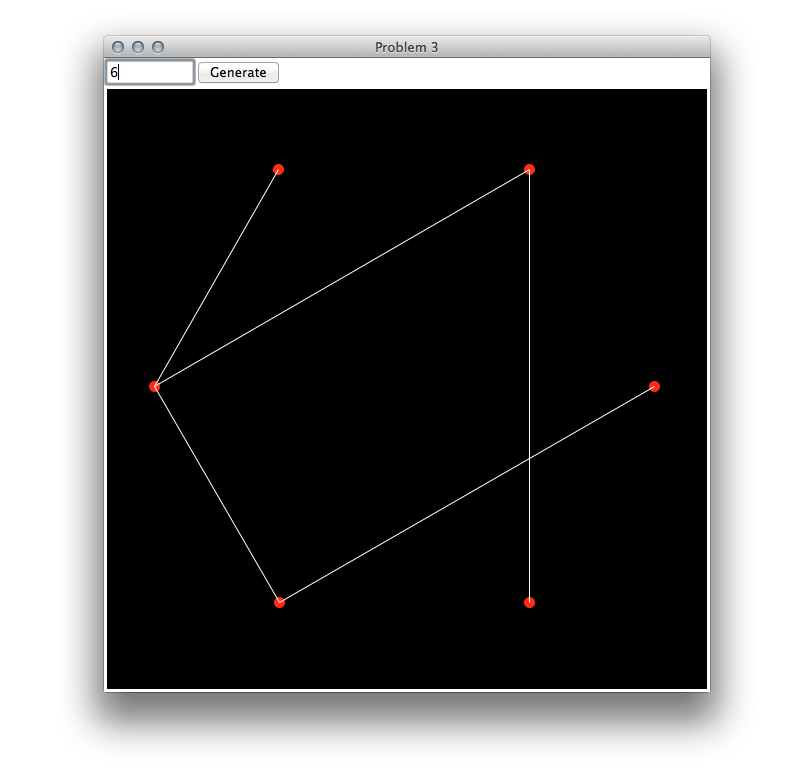
\includegraphics[width=6in,trim=1in 1in 1in 1in]{include/prob3gui.png}
    \caption{GUI for Problem 3}
    \label{fig:include_prob3gui}
\end{figure}
In Figure \ref{fig:include_prob3gui} we see that there are a total of 5 edges, which should be defined by the adjacency matrix
\begin{equation}\label{eq:adjM}
    A = 
    \begin{bmatrix}
        0 & 0 & 1 & 0 & 0 & 0 \\
        0 & 0 & 0 & 0 & 0 & 1 \\
        1 & 0 & 0 & 1 & 0 & 0 \\
        0 & 0 & 1 & 0 & 1 & 1 \\
        0 & 0 & 0 & 1 & 0 & 0 \\
        0 & 1 & 0 & 1 & 0 & 0 
    \end{bmatrix}
\end{equation}
We leave it as an exercise to the reader to verify that the adjacency matrix shown in Eq. \ref{eq:adjM} is represented in Figure \ref{fig:include_prob3gui}.
% subsection results (end)
% section tkinter_gui_for_adjacency_matrix (end)